\label{sect:mgt}

\eucommentary{Will get help from Orsay's grant services}

\eucommentary{Describe the organizational structure and the decision-making
(including a list of milestones (table 3.2a)).\\
Explain why the organizational structure and decision-making mechanisms are
 appropriate to the complexity and scale of the project.\\
Describe, where relevant, how effective innovation management will be
addressed in the management structure and work plan.\\
Describe any critical risks, relating to project implementation, that
the stated project's objectives may not be achieved. Detail any risk
mitigation measures. Please provide a table with critical risks
identified and mitigating actions (table 3.2b).}


\begin{tabular}{|m{.4\textwidth}|c|m{.5\textwidth}|}\hline
  Risk & Level with and without mitigation & Mitigation measures\\\hline

  \TODO{details on this risk?}
  Finding highly qualified personnel to hire & High/Medium &
  Great care was taken identifying pool of candidates to hire from,
  and coordinating with currently running projects to rehire personnel
  with strong track record. Typically, we will rehire European
  postdocs that are currently funded by the Sloan grant to work on
  Jupyter in California and wish to come back to Europe.\\\hline

  Drowning postdocs under technical work & High/Low &
  Great care will be taken in distinguishing PhD and postdocs that
  wish to pursue an academic carrier and full time developers, and
  assigning to the former tasks with a strong research aspect that
  will lead to publications (typically in computer science).\\\hline

  slmhnlnhfnhs&hsfhs&ghshsh\\\hline
\end{tabular}


%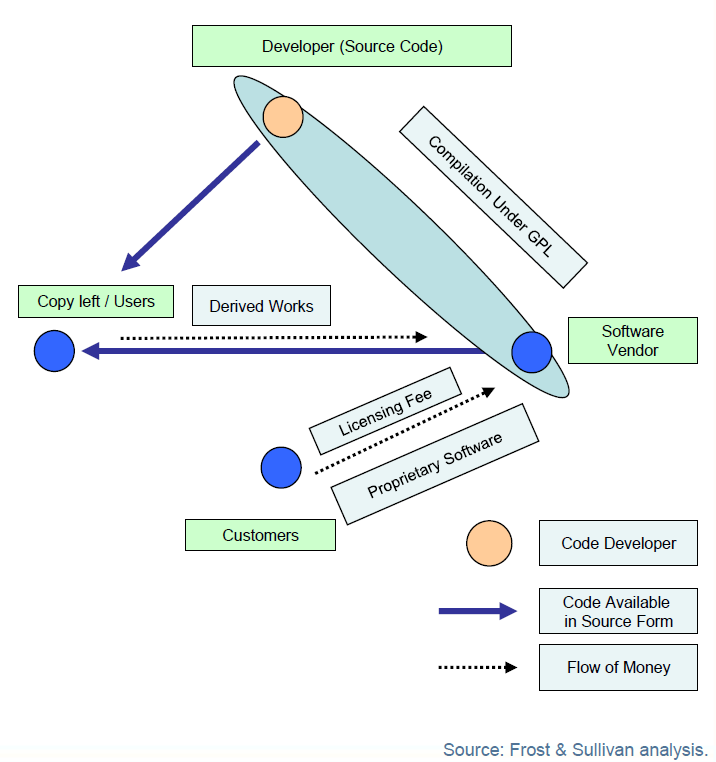
\includegraphics[width=.94\textwidth]{Pictures/Impact-img1.png}


\TODO{An open source architecture allows risk sharing: collaborating
  in the early stages of research could help an early detection, and,
  by consequence, reducing risks.}

\TODO{But: since Open Source softwares are freely accessible, security
  and privacy issues are a concern. Anytime a resource is shared,
  there is greater risk of unauthorised access and contaminated data.
  Providers must demonstrate security solutions, which should include
  physical security controlling access to the facility and protection
  of user data from corruption and cyber attacks.}

